\chapter{METHODOLOGY}
This chapter describes the methodology adopted to develop a Nepali Speech-to-Text system using the Whisper model. Describes the data processing pipeline, the architecture of the Whisper model, and the integration of various modules, including audio pre-processing, feature extraction, inference, and result generation.

\section{Block Diagram}
The block diagram below shows the complete workflow for converting spoken Nepali to text using a Whisper-based model.

\begin{figure}[H]
	\centering
	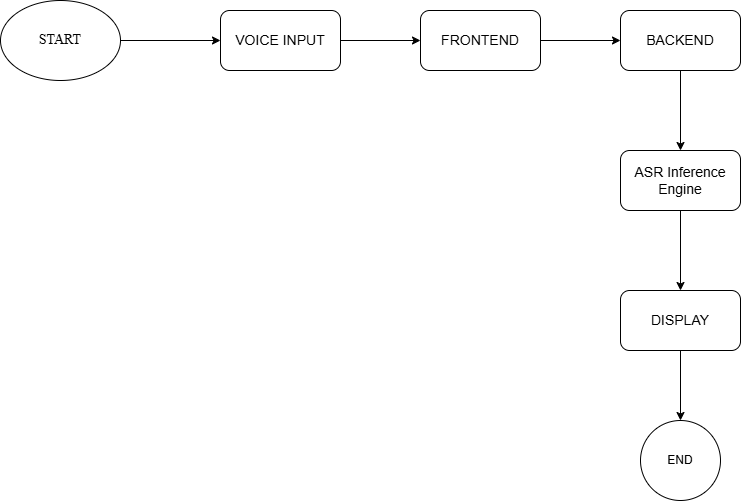
\includegraphics[width=0.90\textwidth]{"Images/deep.png"}
	\caption{Block Diagram of Speech-to-Text System}
	\label{fig:BlockDiagram}
\end{figure}
\begin{figure}[H]
	\centering
	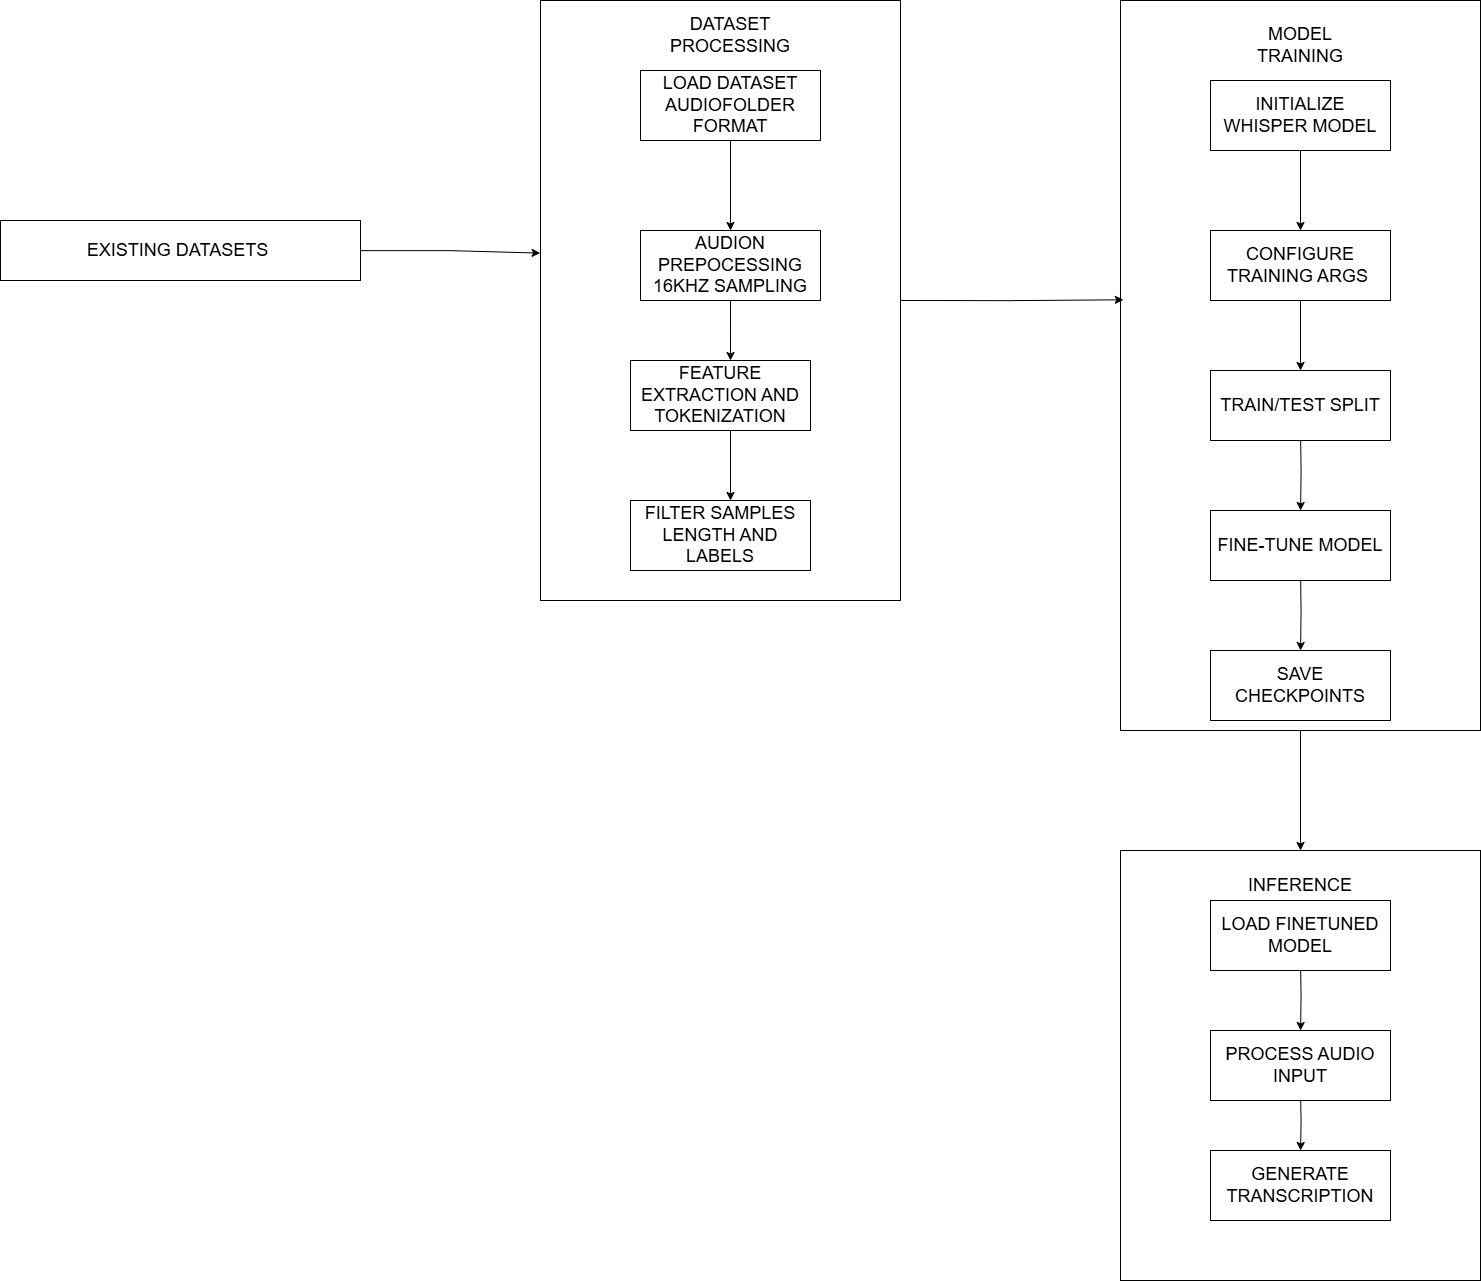
\includegraphics[width=0.90\textwidth]{"Images/finenew.png"}
	\caption{Block Diagram of Fine-tuning pipeline}
	\label{fig: BlockDiagram for Fine-tuning pipeline}
\end{figure}

According to Figure \ref{fig: BlockDiagram}, the speech input is first captured via a microphone. We use a K15 microphone module that consists of an audio capture,  transmitter, and receiver that takes in the audio input.

The frontend, made using React.js js captures the voice input audio. Then it converts it to a blob. The data in the input is taken in the form of a .wav file. The input can be of any length as it is dynamic. The input is taken based on the start and stop buttons provided in the frontend. 

The backend API is created using Flask, which receives the audio and saves the .wav file temporarily, and sends it to the ASR inference engine.
6
ASR inference engine
It is the core of the project. It includes the fine-tuned Whisper-Small for the Nepali ASR model.

 

\textbf{Model Selection:} The model selected for the fine-tuning is a whisper-small model, which is a transformer-based encoder-decoder architecture built by OpenAI. It is trained on a vast dataset that consists of approximately 680,000 hours of multilingual and multitasked supervised data, out of which 117,000 hours are of non-English language. This model is trained on extensive multilingual datasets, which have produced better performance across various languages like English, Nepali, Hindi, etc. It provides a significant improvement over other models for low-resource languages like Nepali, yielding better transcription accuracy. 


 \textbf{Preprocessing steps:} 
 \subsection{ Processor setup} 
 Whisper utilizes a custom WhisperProcessor, which integrate two key components.
 \subsubsection{1. Whisper feature extractor:} It processes the raw audio waveforms taken as input into log\_MEL spectrograms, the input representation used by the whisper model. It performs the audio resampling that ensures the audio is 16 kHz. Data normalization scales audio to a standard range, i.e, (-1 to 1). Also, padding is performed, which standardizes the spectrogram length to a 30-second chunk.\\

 \subsubsection{2. WhisperTokenizer:} It tokenizes the Nepali text into subword units compatible with the whisper decoder. It includes tokens for language identification, timestamps, and task prompts. In our case (eg: ne for Nepali language).\\

 \subsubsection{3. WhisperProcessor (End to End processing):} 
 It combines the features of WhisperProcessor and whisperTokenizer into a single interface. It converts the speech to a Spectrogram through a feature extractor. It converts the text to the tokens via the tokenizer and does the post-processing in which the model prediction is decoded back to the text.

 The processor and essential files like tokenizer\_config.json, vocab.json, etc., are saved locally. 

 \subsection{Dataset:} The dataset used in our project is iamTangsang/OpenSLR54-Nepali-ASR dataset loaded using Hugging Face datasets. It consists of nearly 20.5 hours of .wav format data with the sampling rate of 16 kHz, which is the ideal format for our ASR task. It consists of 10k to 15k unique words covering all the phonemes. It consists of 108866 total samples in the dataset. Each of the entries includes the utterance(i.e, the raw audio) and the transcription i.e (Ground truth).

\subsection{Feature preparation:} IN the feature preparation, we load the audio using librosa and resample the audio to 16 kHz. It is then converted to 80-bin log\_mel Spectrograms using whisperFeatureExtractor. It uses the WHisperTokenizer to convert Nepali text to Token IDs. It returns a dict with input\_features and labels. The output is forced to be in PyTorch tensors instead of numpy for compatibility with the PyTorch-based models like Hugging Face's Whisper. The processed data is uploaded to Hugging Face Hub.

 \subsection{Model architecture:} The base model WhisperFor ConditionalGeneration uses: \\
 \textbf{Encoder:} It processes log-Mel spectrograms \\
 \textbf{Decoder:} Predicts the transcription in target language tokens using the causal attention. 
 The fine-tuning focuses on adjusting decoder weights for improved transcription in Nepali. \\
 \subsection{Data Collation:} We create a custom data collator that prepares variable-length audio-text batches so that the batches are uniform. Also, we add the attention masks, which tell the model which part is real data and which part is padding(so it ignores the padding). It is crucial to create an exact format compatible with the model. \\
 \subsection{Training configuration:}
 The training is managed using the Hugging Face trainer with the following statistics:\\
 \textbf{Batch size:} 8 for training, 16 for evaluation\\
 \textbf{learning rate :} 5e-5\\
 \textbf{Mixed precision(FP16):} \\
 Epochs:5\\
 Data split: 80\%training and 20\% testing \\
 Evaluation strategy: Every epoch \\
 Logging: Tensorboard integration for monitoring\\
 

 \subsection{Evaluation metric:} The evaluation is done using the word error Rate(WER).
 The formula is:\\
 \begin{equation}
     \textbf{WER} = \frac{Substitutions (S) + Deletions (D) + Insertions (I)}{ Total Words in Reference (N)}
 \end{equation}

              

Substitutions (S): Wrong words (e.g., model says "काठमाडौं" instead of "काठमाण्डौ").\\
Deletions (D): Missing words (e.g., model skips "भएको").\\
Insertions (I): Extra words (e.g., model adds "हो" when not spoken).\\
Total Words (N): Number of words in the correct reference text.\\

It is computed by the output of the model with the reference transcriptions.

\subsection{Training and evaluation:} Our model uses the Hugging Face's trainer, which automates the entire training loop that handles the batch processing(Splitting the data into batches), Gradient updates (adjusting the model weights ), learning rate scheduling(Dynamically adjusting the learning rate), etc. We use Tensorboard to track the WER, Loss, and gradients in real-time.

Save and deployment: The model is then saved and pushed to Hugging Face. 

\section{Working principle}
Whisper works by converting speech into text using a sequence-to-sequence Transformer model. The process begins with the input audio being transformed into a mel-spectrogram, a visual representation of sound over time. This spectrogram is then passed into the encoder, which uses multiple Transformer layers to extract meaningful features from the audio. These features capture important information such as phonetics, timing, and speaker characteristics. The decoder then takes these encoded features and generates the output text one token at a time using autoregressive decoding, where each new token is predicted based on the previous ones. The model uses attention mechanisms to focus on the most relevant parts of the audio during transcription. Unlike models that use CTC loss for alignment, Whisper is trained in an end-to-end manner using paired audio and text data, allowing it to learn direct mappings without the need for frame-level alignment. This design enables Whisper to perform well across multiple languages and accents, including low-resource languages like Nepali.


% Figure \ref{fig: BlockDiagram} outlines the workflow and logical sequence of the components used in our Speech-to-Text system.

% \begin{figure}[H]
% 	\centering
% 	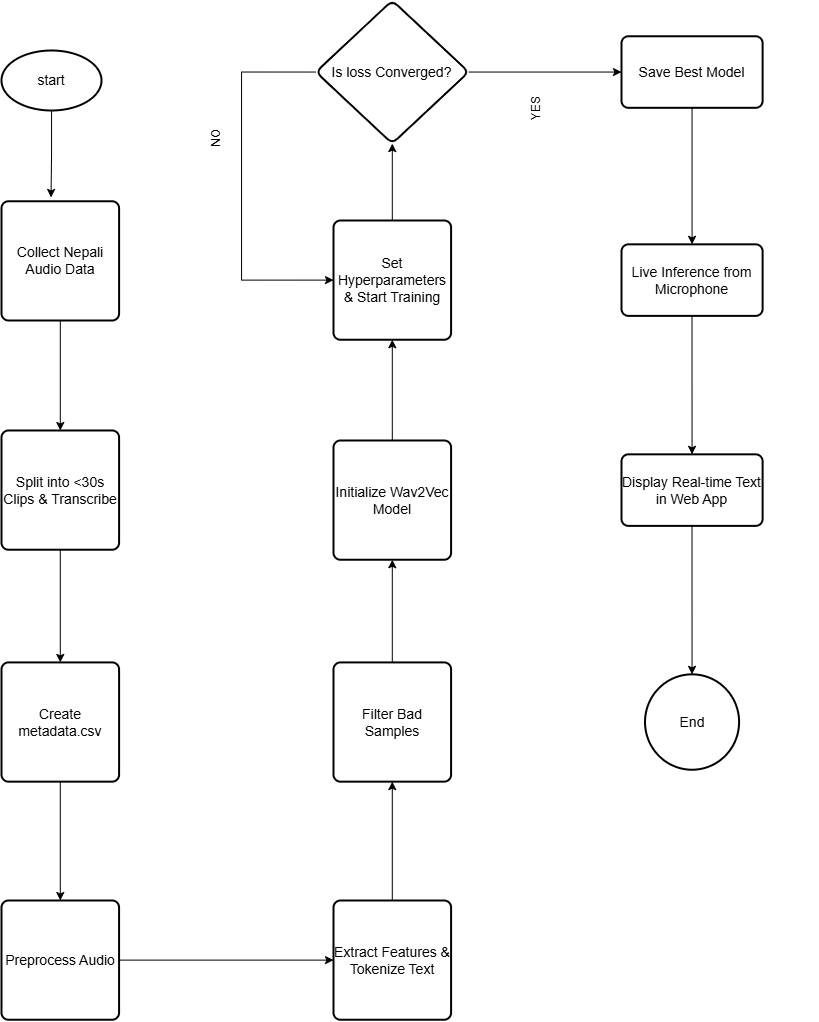
\includegraphics[width=0.92\textwidth]{"Images/5.png"}
% 	\caption{flowchart}
% 	\label{fig:flowchart}
% \end{figure}


\section{Graphical User Interface}
We built a simple GUI to allow users to record, view transcriptions, and download the output. A "Start Recording" button triggers the microphone, and the transcript is displayed in a live text box.

\begin{figure}[H]
	\centering
	\fbox{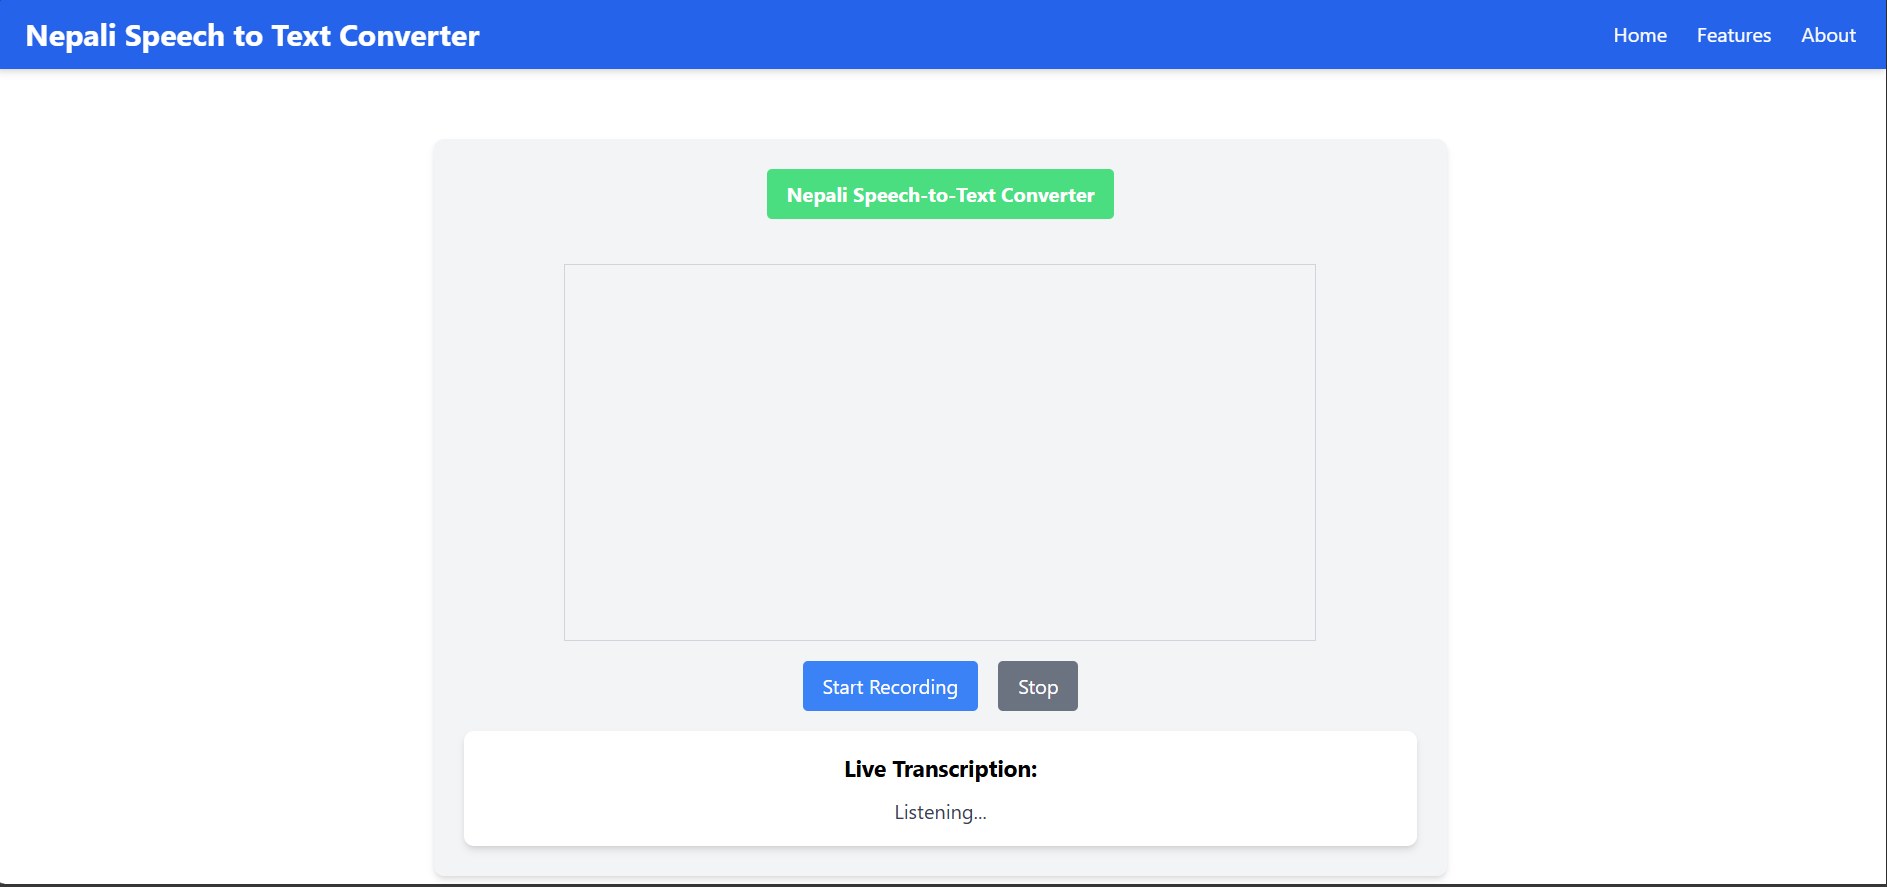
\includegraphics[width=15cm,height=10cm]{"Images/gui.png"}}
	\caption{Graphical User Interface}
	\label{fig:GUI}
\end{figure}

\section{Integration of Whisper with Frontend}
We used Python Flask as a backend to serve the model inference through an API. The GUI (developed using Tkinter or Web Frontend) sends recorded audio to the Flask server, which:
\begin{enumerate}
    \item Accepts the WAV file
    \item Runs Whisper transcription
    \item Returns the transcribed Nepali text
\end{enumerate}

This ensures smooth, real-time integration between the machine learning model and the user interface.



\section{Tools and Techniques}
\subsection{Hardware}
\subsubsection{Microphone Module}
The microphone module captures audio input from the environment, converting sound waves into digital signals. It consists of a microphone sensor, amplifier circuitry, and connectors for interfacing with the Model, enabling real-time audio capture.

\begin{figure}[H]
	\centering
%	\fbox{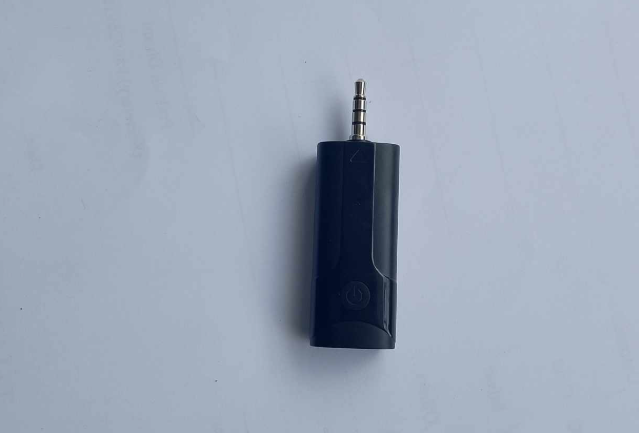
\includegraphics[width=15cm,height=10cm]{"Images/h1.png"}}
	\fbox{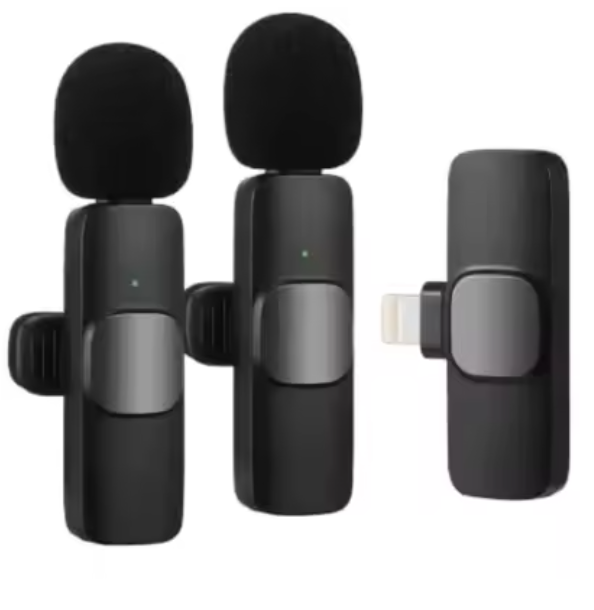
\includegraphics[width=15cm,height=10cm]{"Images/h3.png"}}
	\caption{Microphone}
	\label{fig:MIC}
\end{figure}

% pic


\subsection{Software}
\subsubsection{Python}
Python, a versatile programming language, facilitates the development of software components. Python scripts control hardware interfaces, implement speech recognition algorithms, and manage system behavior, enabling seamless integration and functionality. 

\subsubsection{TensorFlow}
TensorFlow, a Deep Learning framework, powers the speech recognition model. It enables the creation and training of neural network architectures capable of accurately transcribing Nepali speech into text. Additionally, libraries such as pandas, numpy, and matplotlib complement Python's capabilities, facilitating data manipulation, numerical computation, and visualization 
for system optimization and analysis. 
\subsubsection{Hugging Face}
Hugging Face is an open-source platform and company that provides powerful tools and resources for natural language processing (NLP) and machine learning (ML). It is best known for its Transformers library, which offers pre-trained models like GPT, BERT, and T5, enabling developers to easily integrate state-of-the-art NLP capabilities into their applications. Hugging Face simplifies tasks like text classification, translation, summarization, and question answering by offering intuitive APIs and pretrained models that can be fine-tuned for specific use cases. Beyond NLP, Hugging Face supports vision and multimodal tasks, making it versatile for various AI applications. It also fosters a vibrant community-driven ecosystem, where developers and researchers share models and datasets through the Hugging Face Hub. By democratizing access to advanced ML technologies, Hugging Face accelerates innovation and lowers the barrier to entry for AI development. 
